\documentclass[12pt,oneside,a4paper]{article}
\usepackage[table]{xcolor}
\usepackage{graphicx}
\usepackage{amsmath}
\usepackage{fancyhdr}
\usepackage{hyperref}

\begin{document}

\title{Rapport Q-Learning Space Invaders \\ G1I0M3 \\ Étude de l'impact de gamma sur les résultats}

\author{Julien Molinier, Maxime Leras}
\date{7 Mai 2020}
\maketitle\thispagestyle{empty}

\newpage    
\clearpage
\thispagestyle{empty}
\renewcommand*\contentsname{Sommaire}
\tableofcontents
\newpage

\pagestyle{fancy}
\cfoot{\thepage}
\fancyhead{}
\fancyhead[R]{\leftmark}

\pagenumbering{arabic}
\section{Introduction}
\paragraph{}
    Space Invaders est un jeu vidéo d'arcade sorti en 1978. Le principe
    est simple : détruire des vagues d'aliens se déplaçant horizontalement
    grâce à des tirs.
    Le Q-Learning est une technique d'apprentissage automatique
    interéssante pour ce type de jeu car elle ne nécessite aucun modèle 
    initial de l'environnement.
\paragraph{}
    Ce rapport a pour but d'étudier l'impact du paramètre $\gamma$ sur 
    les résultats de l'apprentissage (facteur d'actualisation qui détermine 
    l'importance des récompenses futures).

\section{Description de l'environnement de jeu}
\subsection{Description de l'état du jeu}
\paragraph{}
À chaque étape du jeu, gym atari renvoie 4 valeurs : 
L'objet {\it{observation}} qui ici est une image à l'instant {\it{t}}, le réel {\it{reward}} qui
prend différentes valeurs selon les bonnes ou mauvaises actions du joueur,
le booléen {\it{done}} qui détermine si la partie en cours est terminée ou non et
le dictionnaire {\it{info}} qui peut contenir des informations supplémentaires
par exemple le nombre de vies restantes dans Space Invaders.\footnote{\url{https://gym.openai.com/docs/}}
\subsection{Les récompenses}
\paragraph{}
Les récompenses par défaut pour {\it{SpaceInvaders-v0}} sont uniquement positives.
Elles sont de 5 pour les aliens de la ligne la plus proche du bas et augmentent de 5 par ligne.
Un bonus violet apparaît parfois au dessus des aliens et donne 200 s'il est touché.

Nous avions pensé ajouter une récompense négative dans le cas d'une vie perdue afin de peut-être
permettre un lien entre les tirs des aliens et le fait de perdre. Nous pensions aussi lisser les
récompenses notamment le bonus qui est très rare et crée des fortes croissances dans les scores sans que
le lien {\it{action/reward}} ne puisse être fait.

\newpage
\subsection{Traitement des données}
\paragraph{}
La donnée en entrée est une image de 210 par 160 (160 pixels en horizontal et 210 en vertical)
en couleur. Afin de réduire cette entrée, nous avons réduit la taille de cette image.
l'image au strict nécessaire de 80x80 pixels en noir et blanc. Nous avons fait le choix
de ne garder qu'un seul pixel sur 2 en vertical car aucun déplacement vertical n'est possible et 
les tirs d'aliens restent visibles car bien plus longs que 2 pixels (voir Figure 1). Pour les pixels en abscisse,
nous avons du garder la totalité des pixels et non pas un sur deux car les tirs 
ne font qu'un pixel de large et pourraient être totalement invisible s'ils sont sur un pixel impair.

\begin{figure}[h]
    \centering
    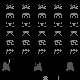
\includegraphics[width=0.5\textwidth] {./processed_image.png}
    \caption{Image après traitement}
\end{figure}

\section{Etude du paramètre $\gamma$}

\end{document}